\chapter{\IfLanguageName{dutch}{Stand van zaken}{State of the art}}%
\label{ch:stand-van-zaken}

% Tip: Begin elk hoofdstuk met een paragraaf inleiding die beschrijft hoe
% dit hoofdstuk past binnen het geheel van de bachelorproef. Geef in het
% bijzonder aan wat de link is met het vorige en volgende hoofdstuk.

% Pas na deze inleidende paragraaf komt de eerste sectiehoofding.
\
\section{Auth technologieën}%
\label{sec:auth-technologieën}
Als eerste onderzoek werd er bekeken welke huidge technologieën er vandaag de dag bestaan en welke de meest gebruikte zijn. Dit omdat er eerst een goede kennis
moet worden gelegd van de huidige technologieën vooraleer er kan worden overgegaan naar de volgende stappen.


\subsection{OAuth 2.0}%
\label{subsec:oauth-2.0}
\autocite{Hardt2012}
OAuth 2.0 wordt gebruikt om toegang tot bronnen te delegeren zonder gebruikersreferenties te delen. Het is een autorisatie framework en wordt dus niet gebruikt voor het authenticeren van gebruikers. Vaak gebruikt om Single Sign On (SSO) en toegangsdelegatie in te schakelen. Kan worden gebruikt in web- en mobiele applicaties en ondersteunt verschillende authenticatiemechanismen.
Dit moet worden geïmplementeerd omdat de service een API gaat aanbieden die toegankelijk is voor applicaties van derden en dus wordt gebruikt voor authentificatie.

\subsubsection{Access Tokens}%
\label{subsubsec:access-tokens}
Access Tokens zijn inloggegevens die worden gebruikt om toegang te krijgen tot bronnen. Access Tokens worden door de autorisatieserver aan de client uitgegeven en worden door de client gebruikt om toegang te krijgen tot bronnen die worden beschermd door de autorisatieserver. Access Tokens zijn bedoeld voor gebruik met bronservers en worden nooit naar autorisatieservers verzonden.

\subsubsection{Refresh Tokens}%
\label{subsubsec:refresh-tokens}
Refresh Tokens zijn inloggegevens die worden gebruikt om Access Tokens te verkrijgen. Refresh Tokens worden door de autorisatieserver aan de client uitgegeven en worden gebruikt om een nieuw Access Tokens te verkrijgen wanneer het huidige Access Token ongeldig wordt of verloopt, of om extra Access Tokens met een identiek of beperkter bereik te verkrijgen. Het uitgeven van een Refresh Tokens is optioneel, ter beoordeling van de autorisatieserver. Als de autorisatieserver een Refresh Token afgeeft, wordt deze meegenomen bij de uitgifte van een Access Token. In tegenstelling tot Access Tokens zijn Refresh Tokens alleen bedoeld voor gebruik met autorisatieservers en worden ze nooit naar bronservers verzonden.
Dit zou kunnen worden geïmplementeerd met een kortere vervaldatum van het Access Token in plaats van een Access Token met een zeer lange vervaldatum, maar toch de black list met Access Tokens gebruiken.
\begin{figure}[h]
  \centering
  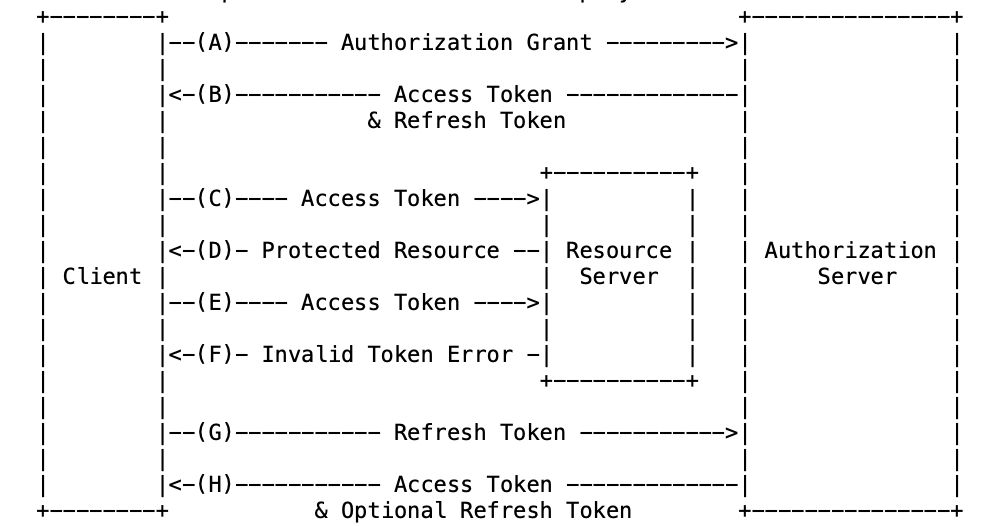
\includegraphics[width=0.5\textwidth]{oauth2.png}
  \caption{OAuth 2.0 verloop}
  \label{fig:example}
\end{figure}

\subsubsection{Client Authentication}
\label{subsubsec:client-authentication}
De client MOET bij elk verzoek NIET meer dan één authenticatiemethode gebruiken.

\subsubsection{Endpoints}%
\label{subsubsec:endpoints}
\begin{enumerate}[label=\textbf{-}]
    \item Authorization Endpoint: \\
    Dit endpoint wordt door de clienttoepassing gebruikt om autorisatie van de resource-eigenaar te verkrijgen. Meestal houdt dit in dat de gebruiker wordt omgeleid naar het autorisatie-endpoint van de autorisatieserver, waar hij/zij kan inloggen en machtigingen kan verlenen aan de clienttoepassing. Na het verlenen van autorisatie leidt de autorisatieserver de gebruiker terug naar de clienttoepassing met een autorisatiecode of toegangstoken.
  
    \item Token Endpoint (optioneel?): \\
    Na het verkrijgen van autorisatie van de eigenaar van de bron, wisselt de clienttoepassing de autorisatiecode uit voor een toegangstoken door een verzoek naar het token endpoint te sturen. Dit endpoint is verantwoordelijk voor het authenticeren van de client en het uitwisselen van de autorisatiecode voor een Access Token. Het token endpoint wordt door de client gebruikt om een Access Token te verkrijgen door de Authorization Grant of Refresh Token te presenteren.
  
    \item Redirection Endpoint: \\
    Dit is niet bepaald een endpoint, maar het is een cruciaal onderdeel van de OAuth-stroom. Het is de URI waar de autorisatieserver de user-agent (meestal een webbrowser) omleidt nadat de resource-eigenaar toegang tot de clienttoepassing heeft verleend/geweigerd. De redirect-URI bevat doorgaans parameters zoals de autorisatiecode of het Access Token. Wanneer een redirect-URI is opgenomen in een autorisatieverzoek, MOET de autorisatieserver de ontvangen waarde vergelijken en matchen met ten minste één van de geregistreerde redirect-URI's(of URI-componenten), als er redirect-URI's zijn geregistreerd. Als de clientregistratie de volledige redirect-URI bevatte, MOET de autorisatieserver de twee URI's vergelijken met behulp van eenvoudige string vergelijking. Als de validatie van een autorisatieverzoek mislukt vanwege een ontbrekende, ongeldige of niet-overeenkomende redirect-URI, MOET de autorisatieserver de eigenaar van de bron op de hoogte stellen van de fout en MOET de user-agent NIET automatisch worden omgeleid naar de ongeldige redirect-URI.
  \end{enumerate}

\subsubsection{Authorization request}%
\label{subsubsec:authorization-request}
De client maakt een verzoek naar de autorisatieserver om autorisatie te verkrijgen. Het verzoek bevat de volgende parameters:
\begin{enumerate}[label=\textbf{-}]
    \item response type: \\
    Deze parameter geeft het gewenste responstype aan. De waarde MOET "code" zijn voor autorisatiecode of "token" voor Access Token.
  
    \item client id: \\
    Deze parameter geeft de client-ID van de clienttoepassing aan. De waarde MOET overeenkomen met de geregistreerde client-ID van de clienttoepassing.
  
    \item redirect uri: \\
    Deze parameter geeft de URI aan waar de autorisatieserver de gebruiker na autorisatie moet omleiden. De waarde MOET overeenkomen met een van de geregistreerde redirect-URI's van de clienttoepassing.
  
    \item scope: \\
    Deze parameter geeft de machtigingen aan die de clienttoepassing wil verkrijgen. De waarde MOET een spatiegescheiden lijst van machtigingen zijn.
  
    \item state: \\
    Deze parameter geeft een willekeurige, niet-voorspelbare waarde aan die door de clienttoepassing wordt gegenereerd. De waarde MOET worden gebruikt om CSRF-aanvallen te voorkomen.
  \end{enumerate}
  En kan er als volgt uitzien:
  \begin{verbatim}
  GET /authorize?response_type=code&client_id=s6BhdRkqt3&state=xyz&redirect_uri=https%3A%2F%2Fclient%2Eexample%2Ecom%2Fcb HTTP/1.1
  Host: server.example.com
  \end{verbatim}

\subsubsection{Authorization reponse}%
\label{subsubsec:authorization-reponse}
De autorisatieserver verleent autorisatie aan de clienttoepassing en leidt de gebruiker terug naar de clienttoepassing met een autorisatiecode of toegangstoken. Het antwoord bevat de volgende parameters:
\begin{enumerate}[label=\textbf{-}]
    \item code: \\
    Deze parameter geeft de autorisatiecode aan die door de autorisatieserver is gegenereerd. De autorisatiecode wordt gebruikt door de clienttoepassing om een toegangstoken te verkrijgen.
  
    \item state: \\
    Deze parameter geeft de waarde van de state-parameter van het autorisatieverzoek aan. De waarde MOET overeenkomen met de waarde die door de clienttoepassing is verstrekt.
  \end{enumerate}
  En kan er als volgt uitzien:
  \begin{verbatim}
    HTTP/1.1 302 Found
    Location: https://client.example.com/cb?code=SplxlOBeZQQYbYS6WxSbIA&state=xyz
  \end{verbatim}

\subsubsection{Error response}%
\label{subsubsec:error-response}
Als het verzoek mislukt vanwege een ontbrekende, ongeldige of niet-overeenkomende redirect-URI, of als de client-ID ontbreekt of ongeldig is, MOET de autorisatieserver de eigenaar van de bron op de hoogte stellen van de fout en MOET de user-agent NIET automatisch omleiden naar de ongeldige redirect-URI.

\subsubsection{Een Access Token vernieuwen}%
\label{subsubsec:een-access-token-vernieuwen}
Als de autorisatieserver een Refresh Token aan de client heeft uitgegeven, doet de cliënt een vernieuwingsverzoek aan het token endpoint.
Indien geldig en geautoriseerd, geeft de autorisatieserver een Access Token uit. Als de verificatie van het verzoek is mislukt of ongeldig is, retourneert de autorisatieserver een foutreactie.
De autorisatieserver KAN een nieuw Refresh Token uitgeven, in welk geval de cliënt het oude Refresh Token MOET weggooien en vervangen door het nieuwe Refresh Token. De autorisatieserver KAN het oude Refresh Token intrekken nadat een nieuw Refresh Token aan de client is uitgegeven. Als er een nieuw Refresh Token wordt uitgegeven, MOET het bereik van het Refresh Token identiek zijn aan dat van het Refresh Token dat door de client in de aanvraag is opgenomen.

\subsubsection{Beveiligingsoverwegingen}
\label{subsubsec:beveiligingsoverwegingen}
\begin{enumerate}[label=\textbf{-}]
    \item Client Impersonation: \\
    Een kwaadwillende client kan zich voordoen als een andere client en toegang krijgen tot beschermde bronnen als de nagebootste client er niet in slaagt of niet in staat is zijn clientreferenties vertrouwelijk te houden.

    \item Access Tokens: \\
    De autorisatieserver MOET ervoor zorgen dat Access Tokens niet door onbevoegde partijen kunnen worden gegenereerd, gewijzigd of geraden om geldige toegangstokens te produceren.

    \item Refresh Tokens: \\
    De autorisatieserver MOET de binding tussen het Refresh Token en de clientidentiteit verifiëren wanneer de clientidentiteit kan worden geverifieerd. Wanneer clientauthenticatie niet mogelijk is, MOET de autorisatieserver andere middelen inzetten om misbruik van Refresh Token te detecteren. De autorisatieserver zou bijvoorbeeld Refresh Token rotatie kunnen gebruiken, waarbij een nieuw Refresh Token wordt uitgegeven bij elke vernieuwingsreactie van het Access Token. Het vorige Refresh Token wordt ongeldig gemaakt, maar behouden door de autorisatieserver. Als een Refresh Token wordt aangetast en vervolgens door zowel de aanvaller als de legitieme client wordt gebruikt, zal een van hen een ongeldig Refresh Token presenteren, dat de autorisatieserver op de hoogte stelt van de inbreuk. De autorisatieserver MOET ervoor zorgen dat Refresh Tokens niet door onbevoegde partijen kunnen worden gegenereerd, gewijzigd of geraden dat ze geldige Refresh Tokens produceren.

    \item Request Confidentiality: \\
    Access Tokens, Refresh Tokens, wachtwoorden voor resource-eigenaren en klantreferenties MOETEN NIET openbaar worden verzonden. De parameters "state" en "scope" MOETEN GEEN gevoelige klant- of resource-eigenaarinformatie in platte tekst bevatten, omdat deze via onveilige kanalen kunnen worden verzonden of onveilig kunnen worden opgeslagen.
\end{enumerate}


\subsection{OAuth 2.0 voor Native Apps}%
\label{subsec:oauth-2.0-voor-native-apps}
\autocite{Denniss2017}
Een native app is een app die door de gebruiker op zijn apparaat wordt geïnstalleerd, in tegenstelling tot een webapp die alleen in de browsercontext wordt uitgevoerd. Apps die zijn geïmplementeerd met behulp van webgebaseerde technologie maar worden gedistribueerd als een native app, de zogenaamde "hybride apps", worden voor het doel van deze specificatie beschouwd als gelijkwaardig aan native apps.
OAuth 2.0-autorisatieverzoeken van native apps mogen alleen worden gedaan via externe user-agents, voornamelijk de browser van de gebruiker. Het andere alternatief is het gebruik van ingebedde user-agents. Deze aanpak heeft veel nadelen, waaronder het feit dat de host-app gebruikersgegevens en cookies kan kopiëren en dat de gebruiker zich in elke app helemaal opnieuw moet authenticeren. Autorisatieverzoeken voor native apps die de browser gebruiken, zijn veiliger en kunnen profiteren van de authenticatiestatus van de gebruiker. Door de bestaande authenticatiesessie in de browser te kunnen gebruiken, is eenmalige aanmelding (SSO) mogelijk, omdat gebruikers zich niet telkens opnieuw hoeven te authenticeren bij de autorisatieserver wanneer ze een nieuwe app gebruiken.
Sommige OAuth-serverimplementaties die ervan uitgaan dat alle clients vertrouwelijke webclients zijn, zullen inzicht moeten geven in openbare native app-clients en de typen redirect-URI's die ze gebruiken om deze best practice te ondersteunen.
\begin{figure}[h]
  \centering
  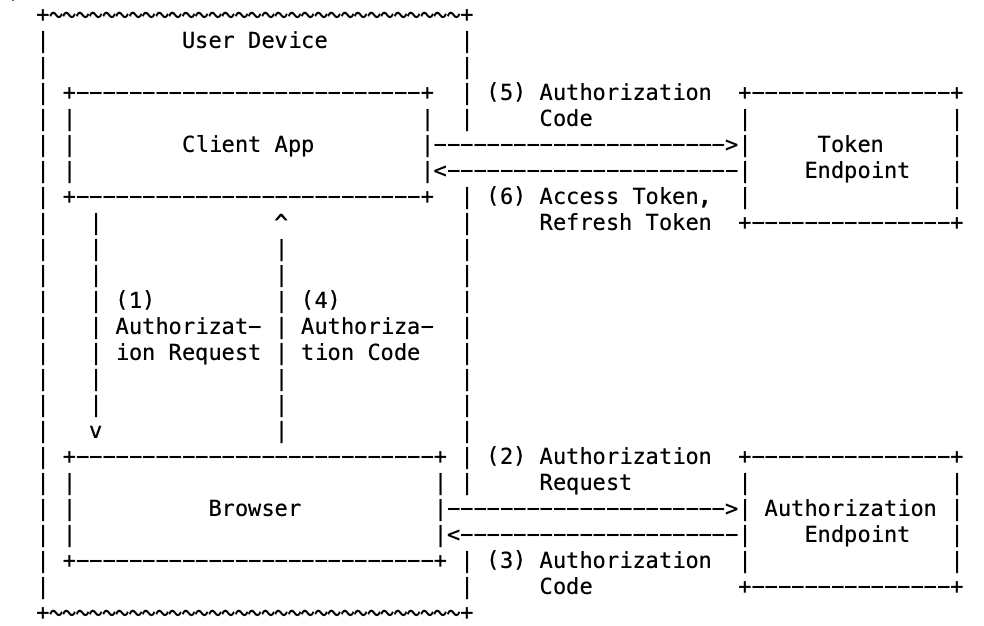
\includegraphics[width=0.5\textwidth]{oauth2_native.png}
  \caption{OAuth 2.0 verloop in native apps}
  \label{fig:example}
\end{figure}
\newline
Dit wordt bereikt door het autorisatieverzoek in de browser te openen en een redirect-URI te gebruiken die het autorisatieantwoord terugstuurt naar de native app.
\newline
\newline
Het ontvangen van de Autorisatiereactie in een Native App gebeurt ook via een redirect URI, er zijn verschillende opties:
\newline
- Omleiding van URI-schema voor privégebruik: nadat de auth-server het verzoek heeft voltooid, wordt deze omgeleid naar de omleidings-URI van de client, com.example.app:/oauth2redirect/example-provider, dit resulteert erin dat het besturingssysteem de native app start en de URI als startparameter.
\newline
- Geclaimde 'https'-schema-URI-omleiding: https://app.example.com/oauth2redirect/example-provider, door de app geclaimde 'https'-schema-omleidings-URI's hebben enkele voordelen vergeleken met andere native app-omleidingsopties, omdat de identiteit van de de bestemmingsapp wordt door het besturingssysteem gegarandeerd aan de autorisatieserver. Om deze reden MOETEN native apps deze waar mogelijk boven de andere opties gebruiken.
\newline
- Loopback Interface Redirection: http://127.0.0.1:51004/oauth2redirect/example-provider, voornamelijk voor desktop-apps die een poort op de loopback-netwerkinterface kunnen openen zonder speciale machtigingen nodig te hebben, kunnen de loopback-interface gebruiken om de OAuth te ontvangen omleiden.


\subsection{OAuth 2.0: Bearer Token gebruik}%
\label{subsec:oauth-2.0-bearer-token-gebruik}
OAuth 2.0 bearer tokens kunnen worden gebruikt in HTTP-verzoeken om toegang te krijgen tot beveiligde bronnen \autocite[p.~{Section 1.0}]{Jones2012}.
Een bearer token is een token dat kan worden gebruikt door iedereen die eigenaar is van het token, zonder dat er bewijs nodig is van het bezit van cryptografisch materiaal \autocite[p.~{Section 1.2}]{Jones2012}.
Er worden drie manieren beschreven om een bearer token in een aanvraag op te nemen: in de Authorization-header, als een formuliergecodeerde body-parameter of als een URI-queryparameter \autocite[p.~{Section 2.1}]{Jones2012}. Als een verzoek mislukt, moet de bronserver een 401-statuscode en een foutcode retourneren, zoals 'invalid\verb|_|request', 'invalid\verb|_|token' of 'insufficient\verb|_|scope' \autocite[p.~{Section 3.0}]{Jones2012}.
Het gebruik van TLS, het valideren van certificaten, het uitgeven van tokens voor de korte termijn en het niet opslaan van tokens in cookies zijn elk sterk aanbevolen \autocite[p.~{Section 5.0}]{Jones2012}.


\subsection{JWT huidige Best Practices}%
\label{subsec:jwt-huidige-best-practices}
Dit document \autocite{Sheffer2020} biedt aanbevelingen voor het op een veilige manier implementeren van JWT's. Ten eerste worden enkele bekende kwetsbaarheden besproken die kunnen optreden bij het gebruik van JWT's, zoals zwakke handtekeningen en onvoldoende handtekeningvalidatie (pagina 2).
Vervolgens worden enkele best practices gegeven om deze problemen aan te pakken. Alle cryptografische bewerkingen moeten bijvoorbeeld worden gevalideerd, er moeten geschikte algoritmen worden gebruikt en de invoer moet worden gevalideerd (pagina's 3-4). Het wordt ook aanbevolen om uitgevers, onderwerpen en doelgroepen te valideren (pagina 5).
Ten slotte wordt aanbevolen om expliciete karakterisering te gebruiken als verschillende typen JWT's kunnen worden gemengd. Ook moeten de validatieregels voor verschillende JWT-typen exclusief zijn (pagina 6).


\subsection{OpenID Connect}%
\label{subsec:openid-connect}
OpenID Connect is een authenticatielaag bovenop OAuth 2.0, een identiteitslaag. Hiermee kunnen klanten de identiteit van de eindgebruiker verifiëren. Definieert een reeks standaardclaims om informatie over de gebruiker over te brengen (overbrengen). Dit moet samen met OAuth 2.O worden gebruikt voor een complete identiteits- en autorisatieoplossing.

OpenID Connect 1.0 voegt identiteitsverificatie toe aan OAuth 2.0 voor clienttoepassingen.
Het maakt het mogelijk om gebruikersinformatie op een veilige en gestandaardiseerde manier te verkrijgen.

Samenvatting: OpenID Connect verifieert identiteiten en biedt veilig basisprofielinformatie via OAuth 2.

Dit document \autocite{Sakimura2014} geeft een uitgebreid overzicht van het OpenID Connect-protocol, dat wordt gebruikt voor gebruikersauthenticatie in webapplicaties. Het begint met het definiëren van de belangrijkste termen en notaties voordat het zich verdiept in verschillende methoden voor gebruikersauthenticatie met behulp van verschillende stromen zoals Autorisatiecodestroom, Impliciete stroom en Hybride stroom. Het proces omvat onder meer stappen als het valideren van verzoeken op autorisatie-eindpunten, het verkrijgen van toestemming van gebruikers en tokenvalidatie op token-eindpunten.

Het document behandelt ook onderwerpen die verband houden met het veilig doorgeven van verzoekparameters, evenals privacyoverwegingen met betrekking tot persoonlijk identificeerbare informatie (PII) en het monitoren van gegevenstoegang. Daarnaast bevat het secties over clientauthenticatiemechanismen; handtekeningen en encryptietechnieken voor het beveiligen van communicatie; offline toegangsbeheer via vernieuwingstokens; serialisatieformaten zoals JSON of querystring enz.; implementatierichtlijnen inclusief verplichte functies voor alle OpenID-providers en vertrouwende partijen.

Verder worden de potentiële veiligheidsrisico's beschreven die verband houden met het gebruik van dit protocol, samen met aanbevelingen om deze risico's effectief te beperken. Ten slotte zijn er IANA-overwegingen die specificeren hoe bepaalde codepunten moeten worden toegewezen binnen registers die door andere specificaties zijn gedefinieerd, terwijl er verwijzingen in de inhoud worden gegeven.

Over het geheel genomen dient dit hulpmiddel zowel de academische nieuwsgierigheid naar moderne protocollen, maar kan het ook praktische inzichten bieden die relevant zijn voor praktijkscenario's voor softwareontwikkeling.
Concluderend zijn de IANA-overwegingen in deze bron van cruciaal belang voor het garanderen van interoperabiliteit en standaardisatie tussen verschillende implementaties van protocollen.

OpenID Connect 1.0 is een identiteitslaag die bovenop het OAuth 2.0-protocol is gebouwd, waardoor klanten eindgebruikers kunnen authenticeren en hun basisprofielinformatie op een gestandaardiseerde manier kunnen verkrijgen. Het breidt OAuth 2.0 uit door het concept van ID-tokens te introduceren, die claims bevatten over de authenticatie van een eindgebruiker door een autorisatieserver bij gebruik van een clientapplicatie.

De OpenID Connect Core 1.0-specificatie definieert de belangrijkste functionaliteit voor het implementeren van authenticatie via OAuth 2.0 en schetst beveiligingsoverwegingen voor het gebruik ervan.

Bovendien wordt ervan uitgegaan dat vertrouwende partijen (clients) de noodzakelijke configuratie-informatie hebben verkregen van OpenID-providers (autorisatieservers), inclusief eindpuntlocaties via detectie of andere mechanismen zoals dynamische registratie.

Over het geheel genomen biedt dit framework interoperabele manieren voor applicaties van derden om de identiteit van gebruikers veilig te verifiëren zonder dat gedetailleerde kennis over de configuraties van individuele autorisatieservers nodig is.
Het is echter belangrijk dat vertrouwende partijen deze configuratie-informatie regelmatig bijwerken en onderhouden om de voortdurende veiligheid en betrouwbaarheid van de verificatie van de gebruikersidentiteit te garanderen.

De inhoud bespreekt de vereisten en procedures voor authenticatie in OpenID Connect. Het benadrukt dat ID-tokens moeten worden ondertekend met JSON Web Signature (JWS) om integriteit, onweerlegbaarheid en eventueel vertrouwelijkheid te garanderen. Het proces omvat verschillende stromen, zoals Autorisatiecodestroom, Impliciete stroom of Hybride stroom.

Met de Authorization Code Flow kunnen clients bijvoorbeeld veilig een ID-token verkrijgen zonder tokens bloot te leggen via een user-agent of kwaadaardige applicaties. Deze stroom ondergaat stappen, waaronder het verzenden van een authenticatieverzoek naar het eindpunt van de autorisatieserver met validatieprotocollen.

Bovendien worden beveiligingsmaatregelen tegen ongeoorloofde toegang tijdens interactie met eindgebruikers benadrukt, waarbij passende standaarden zoals Cross-Site Request Forgery en Clickjacking-beveiligingen worden toegepast door de autorisatieserver.
Het uiteindelijke doel is ervoor te zorgen dat alleen geauthenticeerde en geautoriseerde gebruikers toegang hebben tot de gevraagde bronnen.

De inhoud bespreekt het proces van het verkrijgen van autorisatie en toegangstokens in OAuth 2.0, een protocol voor veilige authenticatie. Het schetst de stappen die betrokken zijn bij interacties tussen een applicatie (relying party), gebruiker en server om toestemming te verkrijgen voor toegang tot beschermde bronnen.

Na een succesvolle authenticatie door de eindgebruiker moet de Autorisatieserver toestemming verkrijgen voordat informatie wordt vrijgegeven aan de Vertrouwende Partij. Dit kan worden bereikt door middel van een interactieve dialoog of eerdere administratieve toestemmingsmechanismen.

Er wordt verder uitgelegd hoe authenticatiereacties en foutreacties worden afgehandeld met behulp van verschillende stromen, zoals de impliciete stroom en de autorisatiecodestroom, waarbij overal duidelijke voorbeelden worden gegeven.

Daarnaast worden tokenverzoeken beschreven die via Token Endpoint van clients naar servers worden verzonden, inclusief validatieprocessen aan beide uiteinden, samen met de afhandeling van foutreacties, indien nodig tijdens deze uitwisseling.
Bovendien behandelt het details over het gebruik van ID-tokens binnen verschillende stromen, zoals impliciete stromen, naast de respectieve validaties die vereist zijn bij het ontvangen ervan van servers na succesvolle uitwisselingen.
Ten slotte biedt het essentiële richtlijnen voor acties aan de clientzijde met betrekking tot deze transacties, waarbij veiligheidsmaatregelen worden gewaarborgd terwijl gevoelige gegevens worden opgehaald. Applicaties die in browsers zijn geïmplementeerd en gebruik maken van scripttalen, volgen specifieke procedures onder Impliciete Stromen die hierin worden uitgelegd, met gedetailleerde verschillen in vergelijking met andere gebruikte protocollen.

Dit zorgt ervoor dat alle acties aan de clientzijde worden uitgevoerd met het hoogste niveau van beveiliging en bescherming voor gevoelige gegevens.

De tekst bespreekt de impliciete stroom en hybride stroom in OAuth 2.0 voor gebruikersauthenticatie, autorisatie en tokenvalidatieprocessen. In het geval van de impliciete stroom wordt gedetailleerd beschreven hoe een authenticatieverzoek wordt gevalideerd en wordt benadrukt dat responsparameters worden toegevoegd aan de fragmentcomponent van een redirect-URI.

Daarnaast worden stappen beschreven zoals het verkrijgen van toestemming van de eindgebruiker en het afhandelen van foutreacties die specifiek zijn voor deze stroom. De inhoud bevat ook instructies voor het ophalen van parametergegevens na de respons aan de clientzijde door gecodeerde waarden van de User Agent te parseren.

Bij het gebruik van de hybride stroom zijn daarentegen vergelijkbare procedures van toepassing, met variaties in sommige aspecten, zoals het gebruik van autorisatie-eindpunten of verificatiemethoden voor de inhoud van ID-tokens, vergeleken met de methoden die in andere stromen worden gebruikt.

Over het algemeen bieden deze secties gedetailleerde technische specificaties met betrekking tot het impliciete stroommechanisme dat verschillende fasen omvat, waaronder aanvraag-/antwoordpatronen over verschillende eindpunten, samen met overwegingen voor gegevensformaten.
Over het algemeen bieden deze secties gedetailleerde technische specificaties met betrekking tot het impliciete stroommechanisme, waardoor een uitgebreid inzicht wordt geboden in het protocol en de implementatie ervan in verschillende scenario's.

De hybride stroom in OpenID Connect omvat de validatie en afhandeling van ID-tokens, tokenverzoeken, tokenreacties, toegangstokens en claims over de eindgebruiker. Wanneer u deze stroom gebruikt voor authenticatie- en autorisatieprocessen tussen clients (applicaties) en identiteitsproviders zoals Google of Facebook:

\begin{enumerate}
  \item De inhoud van een ID-token van zowel het autorisatie-endpoint als het token-endpoint moet op dezelfde manier worden gevalideerd.
  \item Het gebruik van het token-endpoint is vergelijkbaar met dat in de Autorisatiecodestroom.
  \item Validatiemethoden zijn identiek aan die gebruikt in de Autorisatiecodestroom.
\end{enumerate}

Aanvullend:
\begin{enumerate}
  \item[4.] Het specificeert hoe een klant claims kan verkrijgen over de fysieke adressen van eindgebruikers.
  \item[5.] Het beveelt botsingsbestendige namen aan bij het opnemen van aanvullende standaardclaimwaarden.
\end{enumerate}

Verder:
\begin{enumerate}
  \item[6.] De specificatie definieert voor mensen leesbare claimwaarden die in meerdere talen/scripts worden weergegeven volgens de BCP47-richtlijnen voor taaltags.
\end{enumerate}

Het is belangrijk op te merken dat verschillende toegangstokens kunnen worden geretourneerd vanwege verschillende beveiligingskenmerken op eindpunten met verschillende levensduren/bronnen die door hen worden verleend; Er worden ook voorzorgsmaatregelen tegen ongeautoriseerde inlogpogingen via sites van derden geadviseerd.


Het is essentieel om toegangstokens zorgvuldig te beheren en veilig op te slaan om ongeoorloofde toegang of misbruik te voorkomen.

De inhoud omvat de aanbevelingen en vereisten voor taaltagwaarden, afhandeling van UserInfo-claims op een OAuth 2.0 Protected Resource (UserInfo Endpoint), communicatie met het eindpunt met behulp van HTTP-methoden zoals GET en POST, validatie van UserInfo-reacties door clients, gebruik van scope waarden om toegangsrechten op te geven voor toegangstokens in OpenID Connect-clients, waarbij individuele claims worden aangevraagd via parameters voor autorisatieverzoeken.

Volgens de hier genoemde BCP47-richtlijnen wordt aanbevolen om specifieke taaltags alleen te gebruiken als dat nodig is. Het userinfo-eindpunt biedt geverifieerde gebruikersinformatie via JSON-objecten die naam-waardeparen bevatten die bekend staan als 'Claims'. Het specificeert ook beveiligingsmaatregelen zoals TLS-gebruik en ondersteuning voor verschillende methoden, waaronder CORS.

Bovendien zijn scopes gekoppeld aan claimverzoeken terwijl er namens gebruikers een autorisatieserververzoek wordt gedaan; deze definiëren welke bronnen beschikbaar zullen zijn bij tokenpresentatie tijdens toegang tot beschermde broneindpunten vanaf de open ID connect-client.
Ten slotte worden ook het gebruik van vernieuwingstokens en vervaltijden van tokens gedefinieerd om veilige toegangscontrole te garanderen.

De tekst bespreekt het gebruik van de parameter "claims" in OpenID Connect, waarbij wordt gespecificeerd dat de ondersteuning ervan optioneel is voor identiteitsproviders (OP's). Wanneer het wordt ondersteund door een OP en wordt gebruikt door een Relying Party (RP), is het mogelijk om specifieke claims over eindgebruikers op te vragen. Het formaat van deze verzoeken volgt bepaalde regels, waarbij gebruik wordt gemaakt van JSON-codering.

Daarnaast wordt beschreven hoe essentiële en vrijwillige claims worden afgehandeld tijdens authenticatieprocessen. Het legt ook verschillende methoden uit, zoals geaggregeerde en gedistribueerde claims om informatie uit verschillende bronnen op te halen.

Bovendien benadrukt het het belang van het gebruik van stabiele identificatiegegevens die worden verstrekt via specifieke claimwaarden zoals sub en iss, terwijl wordt gewaarschuwd voor het vertrouwen op andere gebruikersspecifieke gegevens vanwege mogelijke veranderingen in de loop van de tijd of tussen emittenten.

Ten slotte introduceert het autorisatieverzoekparameters die ondertekende/gecodeerde authenticatieverzoeken via JWT's mogelijk maken.
  Deze aanpak garandeert de veiligheid en integriteit van authenticatieverzoeken en biedt tegelijkertijd een gestandaardiseerde verificatiemethode.

De ondersteuning voor de verzoekparameter in OpenID Connect Connect is optioneel en het gebruik ervan hangt af van de vraag of de OP (OpenID Provider) deze ondersteunt. Als een RP (Relying Party) deze parameter gebruikt terwijl deze niet wordt ondersteund door het OP, moet er een fout worden geretourneerd. De waarden in een JWT vervangen de waarden die zijn doorgegeven met de OAuth 2.0-syntaxis.

Verzoekobjecten kunnen al dan niet ondertekend zijn en kunnen ook gebruik maken van encryptie met JWE zonder te zijn ondertekend. Wanneer ze worden gebruikt, moeten ze specifieke parameters bevatten, zoals response\verb|_|type en client\verb|_|id, zoals vereist door OAuth 2.0 om de geldigheid te garanderen.

Bovendien zijn er aanvullende overwegingen bij het gebruik van request\verb|_|uri Authorization Request-parameters, waaronder validatiestappen die verder gaan dan de standaard authenticatieverzoeken die worden beschreven in relevante secties van OpenID Connect Connect-specificaties.
Het is essentieel om deze richtlijnen en best practices zorgvuldig te volgen om de veiligheid en integriteit van het autorisatieproces te behouden.

De tekst bespreekt de processen en vereisten voor autorisatieservers bij het omgaan met JSON Web Tokens (JWT) in OpenID Connect. Het schetst dat servers JWT moeten decoderen volgens specifieke standaarden, handtekeningen moeten valideren, indien aanwezig, en autorisatieverzoekparameters moeten samenstellen uit de Request Object-waarde en OAuth 2.0-parameters.

Bovendien introduceert het zelf uitgegeven OpenID-providers als persoonlijke OP's die zelfondertekende ID-tokens uitgeven met behulp van speciale identificatiegegevens. In dit gedeelte wordt beschreven hoe deze providers functioneren zonder dat klanten zich hoeven te registreren of standaard detectieprocedures moeten volgen.
Bovendien worden aanvullende clientauthenticatiemethoden uitgelegd die worden gebruikt tijdens interacties tussen clients en de autorisatieserver op Token Endpoint.

Over het geheel genomen biedt dit document gedetailleerde instructies over het omgaan met verschillende aspecten van open identiteitsprotocollen, zoals validatietechnieken voor decoderingsprocessen, samen met specifieke informatie over de functionaliteit van zelf uitgegeven OP's, die nuttig kunnen zijn voor het begrijpen van beveiligingsmechanismen binnen een identiteitsbeheercontext voor studenten die informatica studeren of cyberbeveiligingsvelden.

De tekst bespreekt het gebruik van JSON Web Signature (JWS) en JSON Web Encryption (JWE) om de berichtintegriteit, authenticatie en vertrouwelijkheid in OpenID Connect-communicatie te garanderen. Er wordt uitgelegd dat door het gebruik van deze technieken berichten zowel kunnen worden ondertekend als gecodeerd voor een betere beveiliging.

Daarnaast wordt uiteengezet hoe de betrokken partijen moeten omgaan met de rotatie van ondertekeningssleutels via JWK Set-publicatie op een specifieke locatie. Het proces omvat het opnemen van sleutel-ID's om aan te geven welke sleutel wordt gebruikt voor validatie. Op dezelfde manier vereist het roteren van encryptiesleutels het publiceren van nieuwe sleutels, terwijl de oude intern behouden blijven voor een soepele overgangsperiode.

Het document behandelt ook de scopes die verband houden met offline toegangsverzoeken in OpenID Connect, evenals richtlijnen voor het vernieuwen van tokens, met voorbeelden die overal in de inhoud worden gegeven.
Bovendien worden syntaxis gedetailleerd met betrekking tot het serialiseren van parameters in verschillende formaten, zoals queryreeksen of JSON-objecten, gebaseerd op specifieke HTTP-verzoektypen zoals respectievelijk GET- of POST-methoden.

De tekst bespreekt de verwerking van OpenID Connect-berichten, waarbij de nadruk specifiek ligt op het vergelijken van waarden in deze berichten met bekende waarden. Het benadrukt de gevolgen voor de veiligheid bij het vergelijken van Unicode-reeksen en specificeert hoe vergelijkingen tussen JSON-reeksen en andere Unicode-reeksen moeten worden uitgevoerd.

Bovendien worden er functies beschreven die zowel Relying Parties (RP's) als OpenID Providers (OP's) naar verwachting zullen implementeren. Deze omvatten verplicht te implementeren functies voor OP's die in twee groepen zijn vermeld: één voor alle OP's en een andere voor 'dynamische' providers.

Het gaat ook in op scenario's waarin vooraf geconfigureerde relaties misschien niet nodig zijn als installaties ervoor kiezen om onverwachte interacties tussen RP's en OP's te ondersteunen zonder een vooraf vastgestelde relatie.

Daarnaast worden overwegingen uiteengezet met betrekking tot het gebruik van autorisatiecode of hybride stromen, het implementeren van nonce-parameterwaardebeschermingstechnieken tegen herhalingspogingen van aanvallers en het garanderen van een veilige verwerking van responsparameters die worden geretourneerd in omleidings-URI-fragmenten door gebruikersagenten met toegang tot cryptografische API's of via validatie. via webserverclients.

Ten slotte worden optionele specificaties benadrukt die de functionaliteit van deze standaard kunnen aanvullen, terwijl wordt verwezen naar relevante beveiligingsoverwegingen uit de OAuth 2.0-standaarden.


Ten slotte belicht het optionele specificaties die de functionaliteit van deze standaard kunnen aanvullen, terwijl wordt verwezen naar relevante beveiligingsoverwegingen uit de OAuth 2.0-standaarden en worden richtlijnen gegeven voor best practices voor een veilige implementatie van de autorisatiecodestroom.

Toegangstokens zijn inloggegevens die worden gebruikt om toegang te krijgen tot beschermde bronnen in het OAuth 2.0-framework. Deze vertegenwoordigen de autorisatie van een eindgebruiker en mogen niet worden blootgesteld aan ongeautoriseerde partijen. Het serverantwoord kan gevoelige clientinformatie bevatten, waardoor deze kwetsbaar wordt als deze openbaar wordt gemaakt. Tot de beperkende maatregelen behoren onder meer het digitaal ondertekenen van antwoorden door de server en het vereisen van een digitale handtekening van clients met behulp van een sleutel die onweerlegbaarheid ondersteunt.

Om aanvallen zoals het vervangen van tokens of het nabootsen van geprivilegieerde gebruikers te voorkomen, wordt doelgroepbeperking voor toegangstokens aanbevolen, samen met een korte geldigheidsduur en het opnemen van tijdstempels in tokens.

OpenID Connect biedt mechanismen via ID Token om tokenvervangingsaanvallen te detecteren en tegelijkertijd problemen aan te pakken die verband houden met meerdere uitgevers per host- en poortcombinatie.

Implementaties moeten het TLS-protocol ondersteunen voor beveiligingsdoeleinden en de richtlijnen volgen uit BCP 195 [RFC8996] (Moriarty et al., maart 2021) voor het verbeteren van de beveiliging van geïmplementeerde services bij het gebruik van TLS.
Het is belangrijk voor organisaties om op de hoogte te blijven van de nieuwste best practices op het gebied van beveiliging en hun implementaties voortdurend dienovereenkomstig bij te werken.

De tekst bespreekt het veilige gebruik van Transport Layer Security (TLS) in online communicatie. Het benadrukt dat servers bij het gebruik van TLS certificaten moeten verifiëren om veilige verbindingen te garanderen. Toegangstokens moeten een korte levensduur hebben en om veiligheidsredenen door de autorisatieserver kunnen worden ingetrokken.

Het behandelt ook belangrijke principes zoals het versleutelen van verzoeken om gevoelige gebruikersinformatie te beschermen, het vermijden van bepaalde soorten HTTP-omleidingen die inloggegevens kunnen lekken, het verkrijgen van expliciete toestemming van gebruikers voordat persoonlijke gegevens worden vrijgegeven, en het beschermen van toegangstokens tegen blootstelling via verschillende stromen.

Bovendien benadrukt het het belang van het respecteren van de privacyregelgeving en het verkrijgen van geldige toestemming voor het verwerken van gebruikersgegevens, terwijl een hoog beveiligingsniveau in verschillende rechtsgebieden wordt gehandhaafd.

Bovendien registreert het specifieke claimparameterfouten met betrekking tot OAuth 2.0 bij de relevante autoriteiten.


Bovendien registreert het specifieke fouten in claimparameters met betrekking tot OAuth 2.0 bij de relevante autoriteiten om eventuele nalevingsproblemen aan te pakken en te corrigeren.

De tekst bespreekt de weergave van algoritme (alg) en sleutelidentificatie (kid) in JSON Web Tokens, met bijzondere aandacht voor het RS256-algoritme. Het benadrukt het belang van het verifiëren en decoderen van ID-tokensegmenten om specifieke claims te verkrijgen. Het document erkent ook bijdragen van verschillende individuen en organisaties aan de specificaties van de OpenID Foundation, terwijl de licentievoorwaarden voor auteursrechten voor reproductie-, ontwikkelings- en implementatiedoeleinden worden benadrukt. Bovendien verduidelijkt het dat de beschikbaarheid van technologie geen goedkeuring of validatie door de stichting impliceert met betrekking tot intellectuele eigendomsrechten die verband houden met het gebruik ervan. Bovendien wordt er melding gemaakt van een patentbelofte met betrekking tot beweerde patentclaims tegen bijdragers en uitvoerders volgens het OpenID Intellectual Property Rights-beleid.

De inhoud legt aspecten uit van het weergeven van algoritmen (alg) en sleutelidentificaties (kid), waarbij de betekenis van RS256 in het verificatie-/decoderingsproces van JWT voor het verkrijgen van specifieke claiminformatie wordt opgemerkt. Het erkennen van de bijdrage van meerdere entiteiten aan de OpenID-specificaties wordt benadrukt naast details over auteursrechtlicenties die materiaalgebruik toestaan, maar zonder een impliciete goedkeuring die de geldigheid of reikwijdte garandeert van IP-rechten met betrekking tot de technologie die in de specificatiedocumenten wordt beschreven.
Het schetst verder het opnemen van een gepatenteerde garantie volgens het OpenID IPR-beleid, samen met het uitnodigen van partijen met relevante auteursrechten/octrooien enz., waarbij het in praktijk brengen van deze specificatie vereist is om ze naar voren te brengen.
Dit benadrukt het belang van transparante en inclusieve samenwerking binnen de OpenID-gemeenschap om een eerlijke vertegenwoordiging en bescherming van intellectuele eigendomsrechten te garanderen.


\subsection*{WebAuthn}%
\label{subsec:webauthn}
WebAuthn is een W3C-specificatie die een webstandaard biedt voor biometrische authenticatie. Het is bedoeld om een veilige en gebruiksvriendelijke manier te bieden om gebruikers te verifiëren zonder dat ze wachtwoorden hoeven te onthouden. WebAuthn maakt gebruik van openbare en privésleutels om gebruikers te verifiëren en biedt een veilige manier om in te loggen op websites en applicaties. Het maakt gebruik van biometrische gegevens zoals vingerafdrukken, gezichtsherkenning en irisscans om gebruikers te verifiëren en biedt een veilige manier om in te loggen op websites en applicaties. WebAuthn is ontworpen om de beveiliging van online accounts te verbeteren en gebruikers te beschermen tegen phishingaanvallen en andere vormen van cybercriminaliteit. Het is een open standaard die wordt ondersteund door alle grote webbrowsers en platformen en wordt gebruikt door bedrijven over de hele wereld om hun online accounts te beveiligen. WebAuthn is een belangrijke stap voorwaarts in de strijd tegen cybercriminaliteit en biedt een veilige en gebruiksvriendelijke manier om gebruikers te verifiëren en hun online accounts te beschermen.



\section{Auth aanbieders}%
\label{sec:auth-aanbieders}
In deze sectie worden enkele van de belangrijkste aanbieders van authenticatiediensten besproken, waaronder Auth0, TrustBuilder en meer. Deze aanbieders bieden een reeks diensten en tools om ontwikkelaars te helpen bij het implementeren van authenticatie en autorisatie in hun applicaties. Ze bieden ook ondersteuning voor verschillende authenticatieprotocollen, waaronder OAuth 2.0 en OpenID Connect, en bieden een reeks functies om ontwikkelaars te helpen bij het beheren van gebruikersidentiteiten en toegangscontrole.
De reden waarom we aanbieders bespreken en vergelijken is om inzicht te krijgen in wat er momenteel wordt aangeboden op de markt, zodat de must haves kunnen worden bepaald voor de ontwikkeling van een eigen authenticatieservice of light weight instance (zie later).


\subsection{Auth0}%
\label{subsec:auth0}
Auth0 is a popular Identity as a Service (IDaaS) platform that provides authentication and authorization services. It supports various identity providers, social logins, and multi-factor authentication. Auth0 offers a range of features, including user management, single sign-on, and passwordless authentication. It also provides SDKs and APIs for integrating authentication into web and mobile applications. Auth0 is widely used by developers and organizations to secure their applications and protect user identities. It is known for its ease of use, scalability, and security features.


\subsection{TrustBuilder}%
\label{subsec:trustbuilder}
TrustBuilder is een Belgisch bedrijf dat gespecialiseerd is in Identity and Access Management (IAM) oplossingen. Het doel van TrustBuilder is om organisaties te helpen bij het beheren van de toegangscontrole tot hun digitale middelen, zoals applicaties, gegevens en systemen, op een veilige en efficiënte manier. Het biedt oplossingen voor authenticatie, autorisatie en het beheer van identiteiten, waardoor organisaties de beveiliging kunnen versterken en tegelijkertijd een naadloze gebruikerservaring kunnen bieden. TrustBuilder richt zich voornamelijk op bedrijven in verschillende sectoren, waaronder financiële dienstverlening, gezondheidszorg, overheid en retail.



\section{Light weight OAuth 2.0 Docker image}%
\label{sec:light-weight-oauth-2.0-docker-image}
Uit de vorige onderzoeken concludeerde ik dat auth al veel verder is geëvolueerd dan ik had verwacht. Er zijn veel aanbieders die een breed scala aan diensten aanbieden, van authenticatie tot autorisatie en alles daartussenin. Het is duidelijk dat het implementeren van een eigen auth-service een enorme taak is en dat het waarschijnlijk niet de moeite waard is, maar persoonlijk zou wel een enorme leerervaring zijn.
\newline
\newline
Het volgende dat onderzocht werd was of er light wieght instances bestaan, zoals bijvoorbeeld een Docker Image, die OAuth 2.0 implementeren. Dit zou een goede oplossing zijn voor een kleinere applicatie die geen behoefte heeft aan de uitgebreide diensten die Auth0 en TrustBuilder aanbieden. Het zou ook een goede oplossing zijn voor een ontwikkelaar die wil leren hoe OAuth 2.0 werkt en hoe het kan worden geïmplementeerd in hun eigen applicatie, zonder af te hangen van een derde partij.
\newline
\newline
Natuurlijk bleek dat er al een Docker Image bestaat die OAuth 2.0 implementeert, namelijk Keycloak, Hydra, ORY Oathkeeper en meer.
\newline
\newline
Lijst van vergelijkingscriteria:

\begin{enumerate}
  \item Gebruiksgemak en configuratie: Hoe gemakkelijk is het om de Docker-image in te stellen en te configureren voor je specifieke gebruiksscenario? Worden er duidelijke instructies geleverd?

  \item Ondersteunde OAuth 2.0-functies: Controleer welke functies van het OAuth 2.0 protocol worden ondersteund door de verschillende implementaties. Dit kan onder meer autorisatiecodes, impliciete access tokens, client credentials en refresh tokens omvatten.
  
  \item Ondersteuning voor andere protocollen: Sommige auth server implementaties ondersteunen naast OAuth 2.0 ook andere protocollen zoals OpenID Connect. Het kan handig zijn om te beoordelen welke protocollen worden ondersteund als je behoeften hebt die verder gaan dan alleen OAuth 2.0.
  
  \item Schaalbaarheid en prestaties: Hoe schaalbaar is de auth server? Kan het omgaan met een groot aantal gelijktijdige gebruikers en verzoeken? Zijn er prestatie benchmarks beschikbaar?
  
  \item Aanpasbaarheid en uitbreidbaarheid: Kun je de functionaliteit van de auth server aanpassen of uitbreiden met behulp van plugins of aangepaste code? Hoe gemakkelijk is het om deze aanpassingen te maken?
  
  \item Documentatie en community ondersteuning: Is er uitgebreide documentatie beschikbaar voor de Docker-image en de bijbehorende auth server? Is er een actieve community waar je vragen kunt stellen en ondersteuning kunt krijgen?
  
  \item Beveiligingsfuncties: Welke beveiligingsfuncties biedt de auth server? Wordt er bijvoorbeeld ondersteuning geboden voor multifactor authenticatie, JWT verificatie of integratie met externe identiteitsproviders?
  
  \item Onderhoud en updates: Wordt de Docker-image regelmatig bijgewerkt met bug fixes en beveiliging patches? Hoe actief is de ontwikkeling van de auth server?
  
  \item Beschikbaarheid van integraties: Controleer of de auth server integraties biedt met populaire frameworks, bibliotheken en platforms die je gebruikt in je applicatie stack.
  
  \item Kosten en licentie: Sommige auth server implementaties zijn gratis en open source, terwijl andere een commercieel licentiemodel hebben. Overweeg welke kosten er zijn verbonden aan het gebruik van de verschillende implementaties en of de licentievoorwaarden aansluiten bij je behoeften.
\end{enumerate}

Laten we enkele populaire Docker-images die OAuth 2.0 implementeren vergelijken, zoals Keycloak, Hydra, en ORY Oathkeeper, op basis van de eerder genoemde criteria:

\begin{enumerate}
  \item Gebruiksgemak en configuratie:
  \begin{itemize}
    \item Keycloak wordt over het algemeen beschouwd als gebruiksvriendelijk met een intuïtieve gebruikersinterface voor configuratie.
    \item Hydra vereist wat meer configuratie, vooral als het gaat om het opzetten van complexe autorisatie flows.
    \item ORY Oathkeeper kan uitdagender zijn om te configureren vanwege de focus op API-gateway functionaliteit, hoewel het krachtige mogelijkheden biedt.
  \end{itemize}
  
  \item Ondersteunde OAuth 2.0-functies:
  \begin{itemize}
    \item Keycloak biedt een breed scala aan functies, waaronder autorisatiecodes, impliciete access tokens, client credentials en refresh tokens.
    \item Hydra is zeer uitgebreid en biedt ondersteuning voor geavanceerde autorisatiefuncties zoals dynamische toestemming verlening.
    \item ORY Oathkeeper richt zich meer op toegangscontrole voor APIs en biedt mogelijk niet dezelfde diepgaande ondersteuning voor OAuth 2.0 als de andere twee.
  \end{itemize}
  
  \item Ondersteuning voor andere protocollen:
  \begin{itemize}
    \item Keycloak biedt ondersteuning voor OpenID Connect en SAML naast OAuth 2.0.
    \item Hydra richt zich voornamelijk op OAuth 2.0, maar biedt ondersteuning voor OpenID Connect.
    \item ORY Oathkeeper is voornamelijk gericht op OAuth 2.0 en JWT verificatie.
  \end{itemize}
  
  \item Schaalbaarheid en prestaties:
  \begin{itemize}
    \item Keycloak kan in grootschalige implementaties prestatieproblemen ondervinden.
    \item Hydra is ontworpen met schaalbaarheid in gedachten en presteert over het algemeen goed in grote omgevingen.
    \item ORY Oathkeeper is lichtgewicht en schaalbaar, maar het ontbreekt mogelijk aan enkele geavanceerde functies voor grote implementaties.
  \end{itemize}
  
  \item Aanpasbaarheid en uitbreidbaarheid:
  \begin{itemize}
    \item Keycloak biedt enige mate van aanpasbaarheid via plugins en themas.
    \item Hydra biedt uitgebreide aanpassingsmogelijkheden met behulp van plugins en aangepaste logica.
    \item ORY Oathkeeper biedt mogelijkheden voor aanpassing, maar het is meer gericht op standaard API-gateway functionaliteit.
  \end{itemize}
  
  \item Documentatie en community ondersteuning:
  \begin{itemize}
    \item Keycloak heeft een grote community en uitgebreide documentatie.
    \item Hydra heeft ook een actieve community, maar de documentatie kan op sommige gebieden ontoereikend zijn.
    \item ORY Oathkeeper heeft een groeiende community, maar de documentatie kan nog wat uitgebreider worden.
  \end{itemize}
  
  \item Beveiligingsfuncties:
  \begin{itemize}
    \item Alle drie de oplossingen bieden robuuste beveiligingsfuncties, waaronder ondersteuning voor multifactor authenticatie en integratie met externe identiteitsproviders.
  \end{itemize}
  
  \item Onderhoud en updates:
  \begin{itemize}
    \item Keycloak en Hydra worden actief onderhouden en bijgewerkt.
    \item ORY Oathkeeper wordt ook regelmatig bijgewerkt, maar de ontwikkeling kan iets minder snel zijn dan bij de andere twee.
  \end{itemize}
  
  \item Beschikbaarheid van integraties:
  \begin{itemize}
    \item Alle drie de oplossingen bieden integraties met populaire frameworks, bibliotheken en platforms, hoewel de diepte van integraties kan variëren.
  \end{itemize}
  
  \item Kosten en licentie:
  \begin{itemize}
    \item Keycloak is gratis en open source.
    \item Hydra en ORY Oathkeeper zijn ook open source, maar sommige functies kunnen onderworpen zijn aan commerciële licenties in bepaalde scenario's.
  \end{itemize}
\end{enumerate}

De zwaktes van veel identiteits- en toegangsbeheer oplossingen, waaronder Keycloak, zijn onder andere:

\begin{enumerate}
  \item Gebruikerservaring
  Een gebied waarop veel identiteits- en toegangsbeheer oplossingen tekortschieten, is de gebruikerservaring bij het inloggen en beheren van gebruikersaccounts. Vaak zijn de standaard authenticatie- en registratie flows te complex of niet goed afgestemd op de specifieke behoeften van een applicatie. Ontwerpen van intuïtieve en aanpasbare gebruikersinterfaces voor authenticatie en account beheer lijkt interessant.
  
  \item Schaalbaarheid en prestaties
  Bij het beheren van grote aantallen gebruikers en verzoeken kunnen sommige identiteits- en toegangsbeheer oplossingen te maken krijgen met prestatieproblemen en schaalbaarheid uitdagingen. Werken aan het optimaliseren van de prestaties en schaalbaarheid van een oplossing lijk een idee, bijvoorbeeld door gebruik te maken van caching, gegevens partitionering en schaalbare infrastructuur.
  
  \item Ondersteuning voor opkomende standaarden
  Hoewel veel oplossingen voldoen aan de gangbare standaarden zoals OAuth 2.0 en OpenID Connect, kunnen ze achterlopen bij het ondersteunen van opkomende standaarden en technologieën die relevant kunnen zijn voor bepaalde toepassingen. Investeren in het verkennen en implementeren van nieuwe standaarden zoals verifiable credentials en decentralized identifiers is een optie.
\end{enumerate}

Het plan is om een nieuw OAuth 2.0 authenticatiesysteem te ontwikkelen dat vergelijkbaar is met bestaande oplossingen zoals Keycloak, Hydra en ORY Oathkeeper, maar met verbeteringen en unieke functies:

\begin{enumerate}
  \item Verbeterde schaalbaarheid en prestaties: Focus op het optimaliseren van de schaalbaarheid en prestaties van het systeem, zodat het gemakkelijk kan omgaan met grote aantallen gelijktijdige gebruikers en verzoeken. Gebruik bijvoorbeeld geavanceerde technieken zoals horizontale schaalbaarheid, caching en asynchrone verwerking om de prestaties te verbeteren.
  
  \item Verbeterde beveiligingsfuncties: Integreer geavanceerde beveiligingsfuncties zoals geavanceerde bedreiging detectie, geografische toegangscontrole, geavanceerde logging en auditing en machine learning-aangedreven anomalie detectie om de beveiliging van het systeem te verbeteren.
  
  \item Gebruiksvriendelijke configuratie en beheer: Zorg voor een intuïtieve gebruikersinterface voor configuratie en beheer, waardoor gebruikers gemakkelijk het systeem kunnen instellen en aanpassen aan hun specifieke behoeften. Bied ook uitgebreide documentatie en ondersteuning om gebruikers te helpen bij het configureren en beheren van het systeem.
  
  \item Verbeterde aanpasbaarheid en uitbreidbaarheid: Maak het systeem zeer aanpasbaar en uitbreidbaar, zodat gebruikers gemakkelijk functionaliteit kunnen toevoegen of aanpassen via plugins, extensies of aangepaste code. Bied een goed gedefinieerde API en ontwikkelplatform voor het bouwen van op maat gemaakte integraties en extensies.
  
  \item Geavanceerde autorisatie- en toestemming beheer: Ontwikkel geavanceerde autorisatie- en toestemming beheer functionaliteit, waaronder ondersteuning voor dynamische toestemming verlening, beleid gebaseerde toegangscontrole, contextuele autorisatie en geavanceerde gebruikersrollen en machtigingen.
  
  \item Verbeterde integraties met externe systemen: Bied uitgebreide integraties met externe systemen en services, waaronder identiteitsproviders, directory services, applicaties en API's. Zorg ervoor dat het systeem gemakkelijk kan integreren met populaire frameworks, bibliotheken en platforms die vaak worden gebruikt door ontwikkelaars.
\end{enumerate}

Door te focussen op deze gebieden kan een OAuth 2.0 authenticatiesysteem ontwikkeld worden dat zich onderscheidt van bestaande oplossingen door verbeterde prestaties, beveiliging, gebruiksgemak en aanpasbaarheid, waardoor het aantrekkelijk is voor gebruikers die op zoek zijn naar een geavanceerde en uitgebreide oplossing.
